\documentclass[11pt,a4paper]{article}

\usepackage[utf8]{inputenc}
\usepackage[T1]{fontenc}
\usepackage[french]{babel}
\usepackage{lmodern}
\usepackage{amsmath,amssymb,mathtools}
\usepackage{mathrsfs}
\usepackage{graphicx}
\usepackage{float}
\usepackage{caption}
\usepackage{geometry}
\usepackage{hyperref}

\geometry{margin=2.25cm}
\graphicspath{{figures_compressed/}}
\setlength{\parindent}{0pt}
\setlength{\parskip}{0.55em}
\captionsetup{font=small}
\hypersetup{
  colorlinks=true,
  linkcolor=black,
  urlcolor=black,
  pdftitle={Les sylphes -- Physique I, filière PC, CCMP 2023},
  pdfauthor={Concours Commun Mines-Ponts}
}

\newcommand{\question}[1]{%
  \par\medskip\noindent\textbf{\(\square\)\ #1.}\quad%
}

\begin{document}

\begin{center}
{\small Concours Commun Mines-Ponts (CCMP) -- Session 2023\\
Filière PC -- Épreuve : Physique I}

\vspace{0.6em}
{\Large\bfseries Les sylphes}
\end{center}

Un formulaire et des données numériques sont fournis à la fin du sujet.
Toutes les applications numériques seront effectuées avec un chiffre significatif.

Les sylphes sont des émissions lumineuses rouges, très intenses et relativement brèves, de l'ordre de quelques centaines de millisecondes, qui se produisent entre le sommet des nuages et l'ionosphère. La majorité d'entre elles se situe entre 40 et 80~km d'altitude. Elles ne sont observées et étudiées que depuis 1990 environ. Certaines de leurs manifestations avaient déjà été rapportées bien avant, mais leur observation depuis la Terre est difficile. Les sylphes font partie d'un groupe d'émissions lumineuses qui se produisent au moment des orages. On retrouve dans le même groupe d'émissions les jets bleus et les elfes, voir la figure~\ref{fig:formes}. Ces émissions sont la conséquence de courants électriques importants qui se produisent lors d'une avalanche de créations d'ions et d'électrons. L'initiateur de l'avalanche peut être une particule du rayonnement cosmique. Lors de chocs avec les molécules, les électrons des courants électriques apportent de l'énergie à celles-ci, perdue ensuite en émettant de la lumière visible.

\begin{figure}[H]
\centering
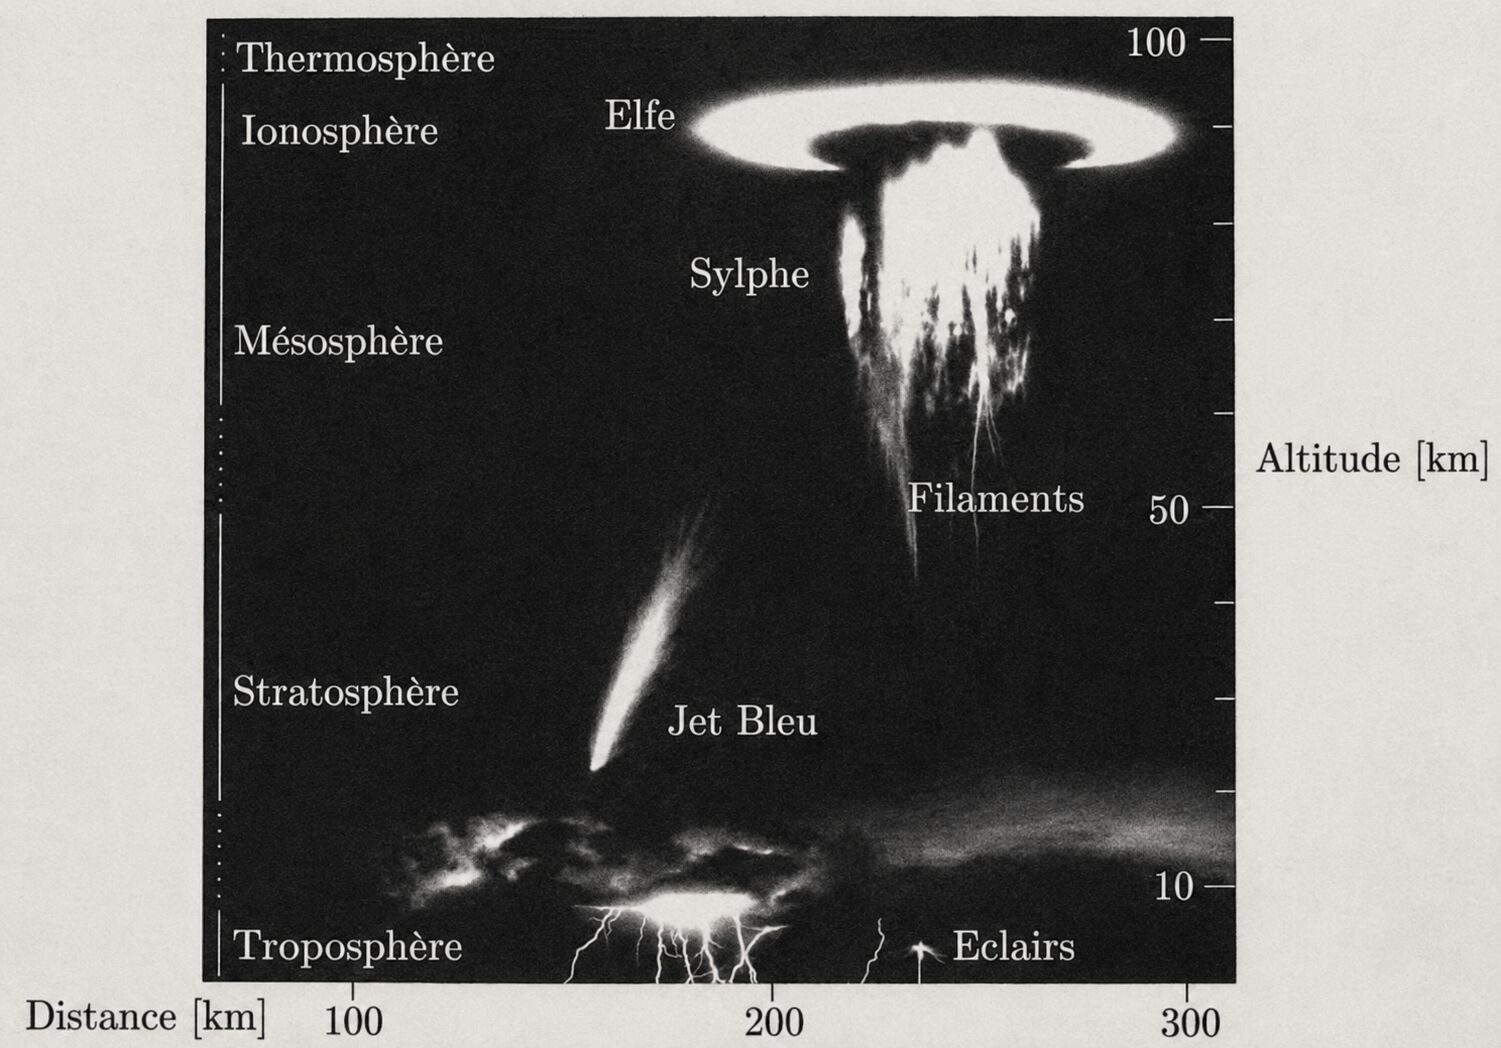
\includegraphics[width=0.78\linewidth]{figure_01.jpg}
\caption{Différentes formes de phénomènes lumineux éphémères atmosphériques.}
\label{fig:formes}
\end{figure}

Ce sujet comporte trois parties largement indépendantes. La première concerne l'observation des sylphes. La seconde étudie des propriétés électriques de l'atmosphère. La dernière partie présente le modèle de la formation avalancheuse du courant à l'origine des sylphes.

\section*{I. Observation des sylphes}

\question{1}
À l'aide des courbes de la figure~\ref{fig:spectre}, justifier la couleur caractéristique des sylphes. Justifier également leur observation difficile depuis la surface de la Terre.

Malgré cette difficulté, des images de sylphes ont été obtenues comme celles de la figure~\ref{fig:photos}, qui ont été observées depuis l'Observatoire du Pic du Midi de Bigorre. Des sylphes y ont été vues au-dessus des Alpes. Le Pic du Midi de Bigorre se situe au milieu de la chaîne des Pyrénées qui s'étend de Perpignan à l'Est jusqu'à Biarritz à l'Ouest, séparant la France de l'Espagne.

\begin{figure}[H]
\centering
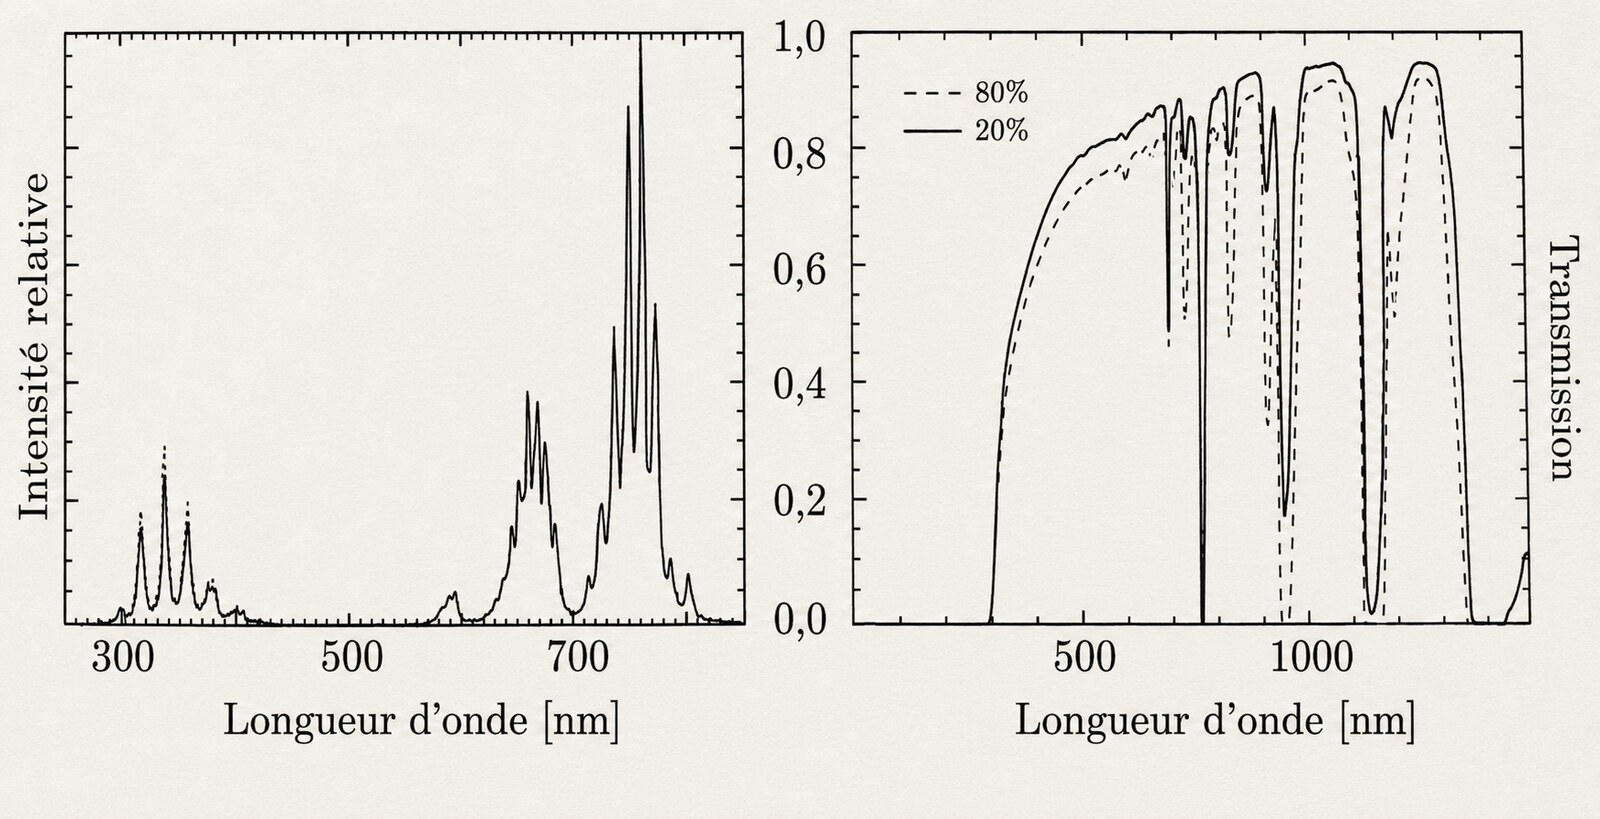
\includegraphics[width=0.88\linewidth]{figure_02.jpg}
\caption{À gauche : spectre d'émission d'un sylphe. À droite : coefficient de transmission de l'atmosphère avec deux taux d'humidité, 20~\% et 80~\%. Ces mesures ont été réalisées par un détecteur au sol placé sous une source située à 80~km d'altitude. Figure tirée de l'article \textit{Spectrum of Red Sprites}, G.~Milikh, J.~A.~Valdivia et K.~Papadopoulos, \textit{Journal of Atmospheric and Solar-Terrestrial Physics}, vol.~60, p.~907--915, 1998.}
\label{fig:spectre}
\end{figure}

Du fait de la rotondité de la Terre de rayon \(R_T\), on s'interroge sur la possibilité de vision de sylphes au-dessus des Alpes.

\begin{figure}[H]
\centering
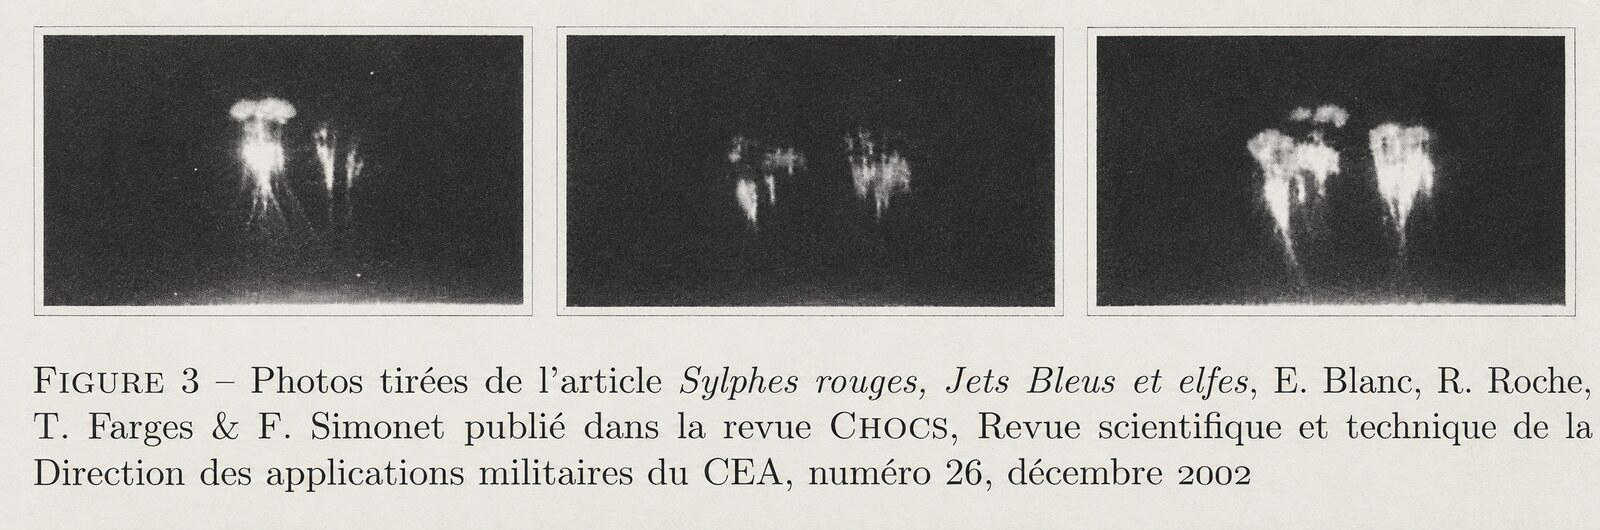
\includegraphics[width=0.88\linewidth]{figure_03.jpg}
\caption{Photos tirées de l'article \textit{Sylphes rouges, jets bleus et elfes}, E.~Blanc, R.~Roche, T.~Farges et F.~Simonet, publié dans la revue \textsc{Chocs}, revue scientifique et technique de la Direction des applications militaires du CEA, numéro~26, décembre~2002.}
\label{fig:photos}
\end{figure}

\question{2}
La distance \(d\) qui sépare à vol d'oiseau le Pic du Midi de Bigorre de la chaîne des Alpes françaises est-elle de l'ordre de 500, 1000 ou 1500~km ?

Sans prendre en compte l'altitude du Pic du Midi de Bigorre, tracer sur un schéma approprié la ligne d'horizon qui en part et qui passe au-dessus des Alpes à une altitude \(h\). En faisant les hypothèses qui s'imposent, exprimer \(h\) en fonction de \(R_T\) et \(d\), puis calculer sa valeur numérique.

Est-il possible de voir des sylphes alpins sans effet de réfraction atmosphérique depuis le Pic du Midi de Bigorre ? Peut-on voir le Mont-Blanc par beau temps ?

Afin de pouvoir observer régulièrement des sylphes et de développer des recherches visant à mieux comprendre leur origine, on utilise depuis 2001, sur la Station spatiale internationale (ISS), deux microcaméras fixées sur un hublot. Les deux caméras observent selon la verticale. L'une de ces deux caméras opère dans le visible tandis que l'autre est équipée d'un filtre de très faible bande passante centré à 761~nm. Sur la figure~\ref{fig:iss}, on peut observer les deux images obtenues lors d'un enregistrement. Cet enregistrement a été réalisé lors d'un orage important.

Sur ces images, l'intensité lumineuse obtenue est exprimée en LSB (\textit{Lower Significant Bit}, unité de mesure spécifique de la caméra). On indique qu'un éclair traditionnel provoque un niveau de 836~LSB sur la caméra opérant dans le visible et donne 30~LSB sur la caméra filtrée.

\begin{figure}[H]
\centering
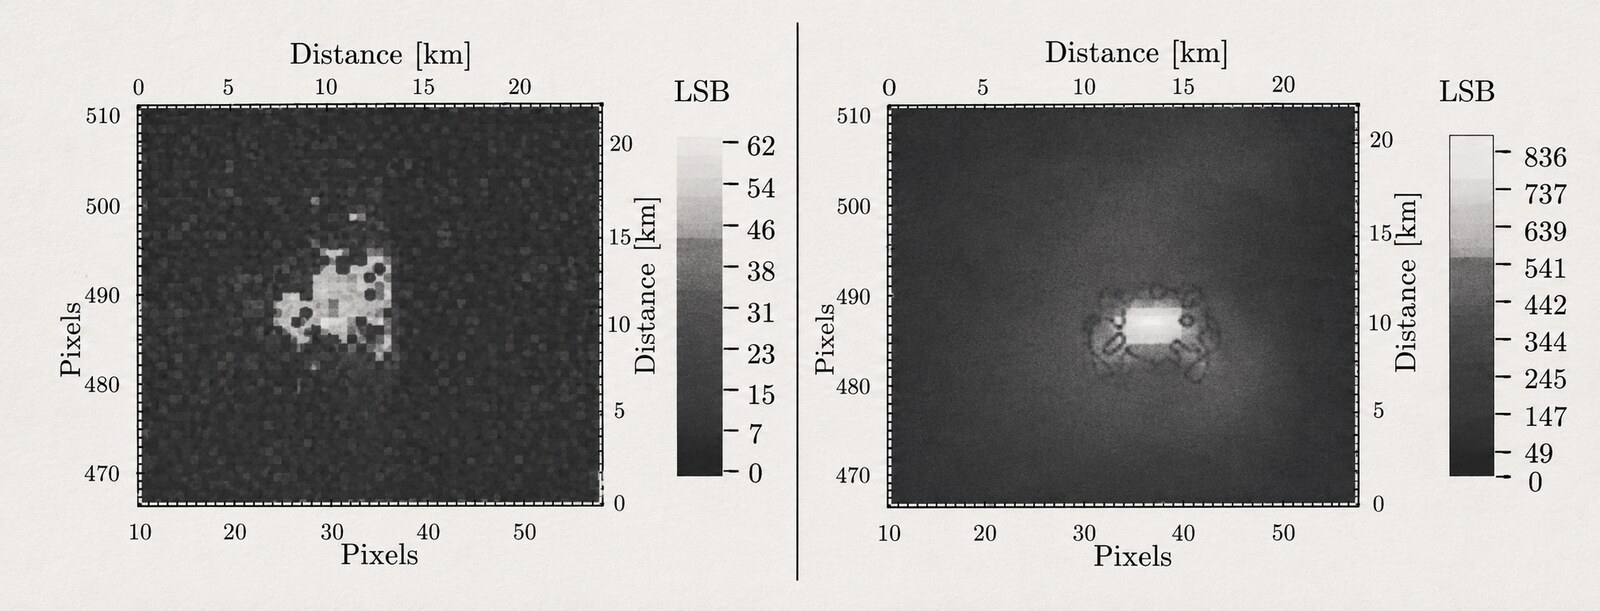
\includegraphics[width=0.86\linewidth]{figure_04.jpg}
\caption{Enregistrements effectués depuis l'ISS par la microcaméra filtrée à gauche et par la microcaméra dans le visible à droite. Un trait noir isole la détection d'un sylphe sur l'image de droite. Figures toujours tirées de l'article référencé en figure~\ref{fig:photos}.}
\label{fig:iss}
\end{figure}

\question{3}
Montrer que l'analyse des deux images de la figure~\ref{fig:iss} prouve bien la détection d'un sylphe.

\question{4}
L'ISS se situe à une altitude \(h_{\mathrm{ISS}}\) d'environ 400~km. Montrer, en utilisant le théorème de Gauss et moyennant certaines hypothèses que l'on précisera, que le champ gravitationnel qu'elle subit est de la forme
\begin{equation*}
G_{\mathrm{ISS}} = g_0 \left(1+\frac{h_{\mathrm{ISS}}}{R_T}\right)^{-2},
\end{equation*}
où \(g_0=9{,}8~\mathrm{m}\cdot\mathrm{s}^{-2}\) est le champ de pesanteur à la surface de la Terre.

\question{5}
Après avoir montré qu'elle est constante, déterminer l'expression \(v_{\mathrm{ISS}}\) de la norme de la vitesse de l'ISS sur son orbite circulaire. Calculer sa valeur numérique en \(\mathrm{km}\cdot\mathrm{s}^{-1}\).

\question{6}
Déterminer l'expression de la période de révolution \(T_{\mathrm{ISS}}\) de l'ISS autour de la Terre et faire le lien avec la troisième loi de Kepler.

\question{7}
Les deux microcaméras de l'ISS ont pour objectif d'enregistrer, lors d'un passage au-dessus d'un orage, la totalité de l'évolution d'un sylphe. Commenter la possibilité et la précision de ces enregistrements. On justifiera les réponses de façon numérique.

Il est difficile d'observer des sylphes depuis la Terre dans le visible, car le dioxygène \(\mathrm{O}_2\) présent dans l'atmosphère absorbe fortement à 762~nm. Toutefois, le dioxygène se raréfie fortement avec l'altitude, ce qui permet des observations au-delà de 40~km d'altitude comme cela est le cas avec l'ISS. Nous allons étudier l'évolution de la pression partielle \(P_{\mathrm{O}_2}(z)\) de dioxygène en fonction de l'altitude \(z\). Le modèle que nous utilisons est le suivant :

\begin{itemize}
\item l'atmosphère est assimilée à un gaz parfait de masse molaire \(M=29~\mathrm{g}\cdot\mathrm{mol}^{-1}\) ;
\item la fraction molaire de dioxygène \(\mathrm{O}_2\) est supposée la même à toute altitude \(z\) et égale à celle à la surface de la Terre, à savoir \(x_{\mathrm{O}_2}=20~\%\) ;
\item l'atmosphère est supposée en équilibre de telle sorte que la loi de la statique des fluides s'y applique et on ne prendra en compte que le poids assimilé à la force gravitationnelle ;
\item la pression à la surface de la Terre est \(P_0=1~\mathrm{bar}\) en \(z=0\), la température \(T_0=290~\mathrm{K}\) ;
\item la température évolue selon la loi \(T(z)=T_0(1-z/\ell)\), avec \(\ell=50~\mathrm{km}\), ce qui limite le modèle nécessairement à des altitudes inférieures à \(\ell\).
\end{itemize}

\question{8}
Rappeler, sans démonstration, l'expression vectorielle de la loi de la statique d'un fluide de masse volumique \(\mu\).

Montrer que la pression atmosphérique \(P(z)\) obéit à l'équation différentielle suivante :
\begin{equation*}
\frac{\mathrm{d}P}{\mathrm{d}z}
= -F(z)\frac{P}{H},
\qquad
F(z)=\frac{1}{(1-z/\ell)(1+z/R_T)^2},
\end{equation*}
où \(H\) est une distance caractéristique que l'on exprimera en fonction de \(R\), \(T_0\), \(M\) et \(g_0\). Évaluer numériquement \(H\) en kilomètres avec un seul chiffre significatif.

En décomposant la fonction \(F\), on peut écrire
\begin{equation*}
F(z)=\frac{\alpha}{1-z/\ell}
+\frac{\beta+\gamma z}{(1+z/R_T)^2},
\end{equation*}
en introduisant les constantes
\[
\alpha=\bigl[1+\epsilon(2+\epsilon)\bigr]^{-1},
\qquad
\beta=\alpha\epsilon(2+\epsilon),
\qquad
\gamma=\frac{\alpha\epsilon}{R_T},
\]
à condition de poser \(\epsilon=\ell/R_T\).

\question{9}
Montrer que dans les conditions du problème on peut prendre \(\alpha\simeq 1\), \(\beta\simeq 2\epsilon\) et \(\gamma\simeq \epsilon/R_T\).

Montrer que la pression \(P(z)\) dans l'atmosphère est alors donnée par
\begin{equation}
P(z)=P_0
\left(\frac{1-z/\ell}{1+z/R_T}\right)^\xi
\exp\left[-\frac{z}{\chi(1+z/R_T)}\right],
\label{eq:pression}
\end{equation}
dans laquelle on précisera l'expression des quantités \(\xi\) et \(\chi\) en fonction de \(\ell\), \(H\) et \(R_T\).

\question{10}
Quelle expression simplifiée de \(P(z)\) proposeriez-vous à la lumière de l'expression précédente et des valeurs des grandeurs engagées dans celle-ci ? À quoi cela revient-il à faire ?

Sur la figure~\ref{fig:pression}, on a représenté sur le même schéma d'une part le modèle de pression de l'équation~\eqref{eq:pression} pour les valeurs adaptées des paramètres et d'autre part la valeur de la pression mesurée par des sondes atmosphériques et spatiales.

\begin{figure}[H]
\centering
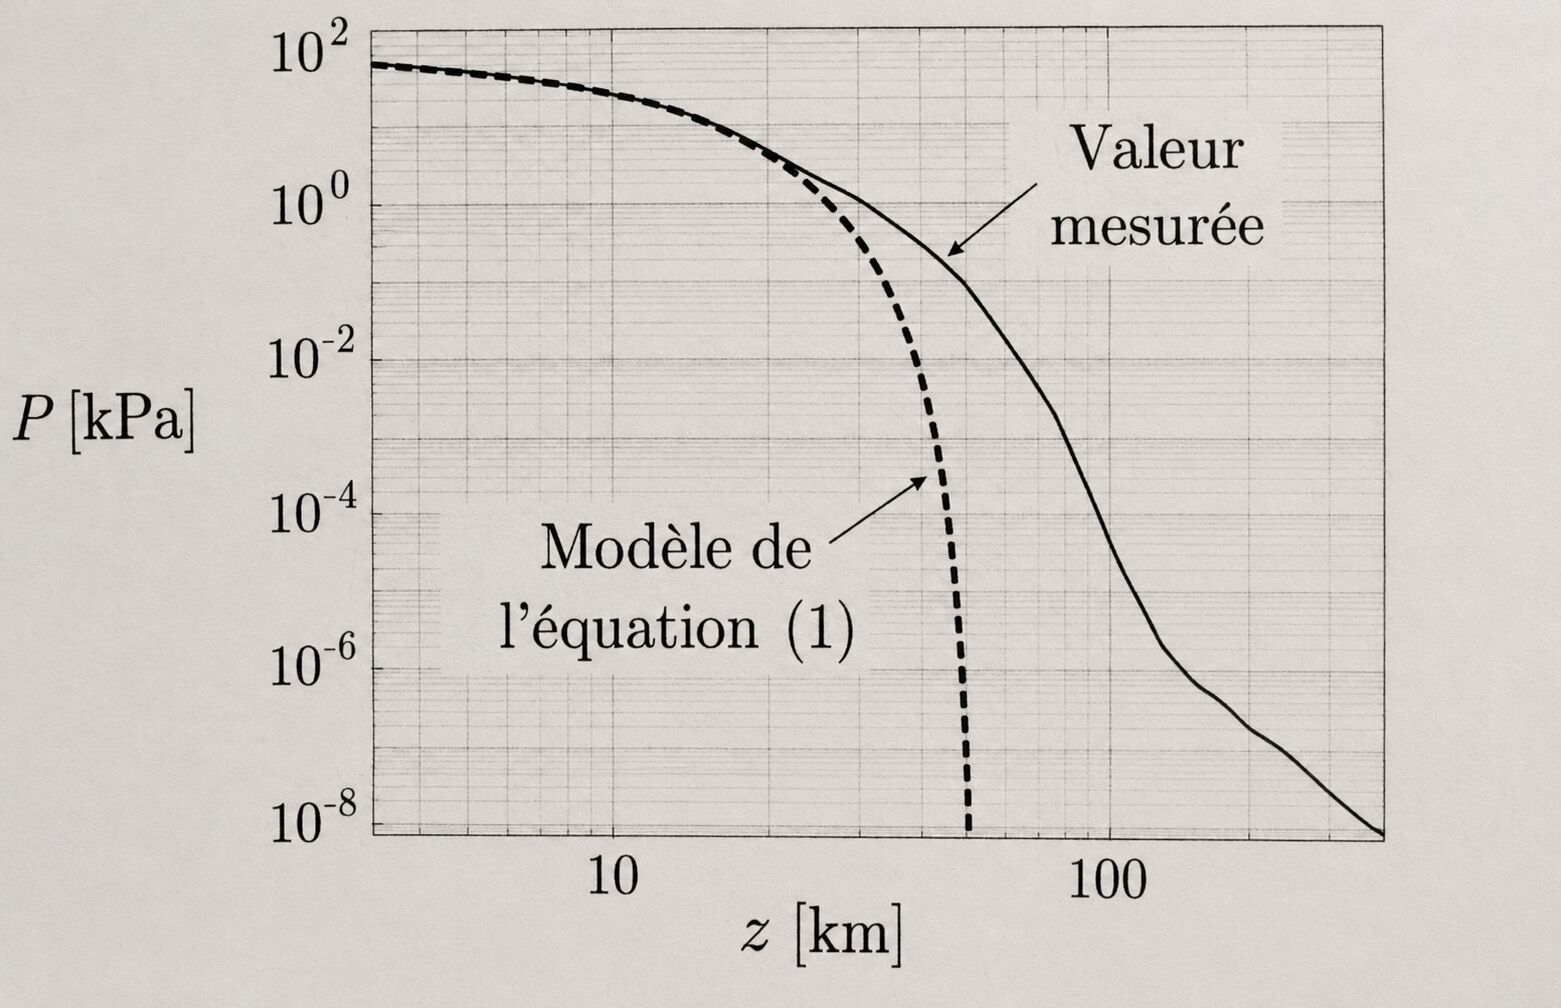
\includegraphics[width=0.72\linewidth]{figure_05.jpg}
\caption{Pression de l'air atmosphérique.}
\label{fig:pression}
\end{figure}

\question{11}
Pour quelle raison principale le modèle étudié cesse-t-il d'être correct à partir d'une altitude de l'ordre de \(z=20~\mathrm{km}\), alors qu'il est censé fonctionner potentiellement jusqu'à 50~km ?

\question{12}
Discuter la possibilité d'observation des sylphes en lien avec la pression partielle en dioxygène depuis la Terre et depuis l'ISS.

\section*{II. Une atmosphère électrique}

L'atmosphère est assimilée à un plasma dans lequel le courant électrique est essentiellement dû à des déplacements d'électrons non relativistes. La densité d'électrons mobiles par unité de volume est notée \(n\), la masse d'un électron \(m_e\), sa charge \(e\).

On étudie, dans un premier temps, la propagation d'une onde électromagnétique plane progressive monochromatique de pulsation \(\omega\), de vecteur d'onde \(\vec{k}=k\vec{e}_z\), polarisée rectilignement et décrite par son vecteur champ électrique à l'instant \(t\),
\[
\vec{E}=\vec{E}_0\exp\bigl(i(\omega t-kz)\bigr),
\qquad
\vec{E}_0\perp\vec{e}_z,
\qquad
\lVert\vec{e}_z\rVert=1.
\]

L'atmosphère est caractérisée par la permittivité diélectrique du vide \(\varepsilon_0\) et par la perméabilité magnétique du vide \(\mu_0\). Dans cette étude, on néglige les chocs que subissent les électrons et leur poids. La seule force agissant sur les électrons est la force de Lorentz.

\question{13}
Montrer que la contribution magnétique de la force de Lorentz sur l'électron est négligeable devant la contribution électrique de cette même force.

\question{14}
Justifier le fait que la contribution des ions au courant électrique est négligeable devant celle des électrons. Déterminer la relation qui existe entre la représentation complexe du champ électrique \(\vec{E}\) de l'onde électromagnétique et celle de la densité volumique de courant \(\vec{j}\) qui résulte de l'interaction entre l'électron et \(\vec{E}\). Donner l'expression de la conductivité complexe du plasma \(\gamma_p\) et commenter cette expression en terme de puissance transférée.

\question{15}
Établir l'équation de propagation du champ électrique \(\vec{E}\). En déduire la relation de dispersion vérifiée par le vecteur d'onde \(k\).

\question{16}
Pour quelle fréquence limite \(f_p\), une onde envoyée depuis la surface de la Terre ne peut plus se propager lorsqu'elle rencontre un milieu où la densité volumique d'électrons est \(n\) ? On détaillera le raisonnement permettant d'obtenir cette limite. Effectuer l'application numérique pour une densité \(n=10^{11}~\mathrm{m}^{-3}\) caractéristique des sylphes.

\question{17}
L'image de la figure~\ref{fig:radar} montre la localisation et le nombre d'échos radar qui reviennent au niveau de l'émetteur. Analyser et commenter cette carte.

\begin{figure}[H]
\centering
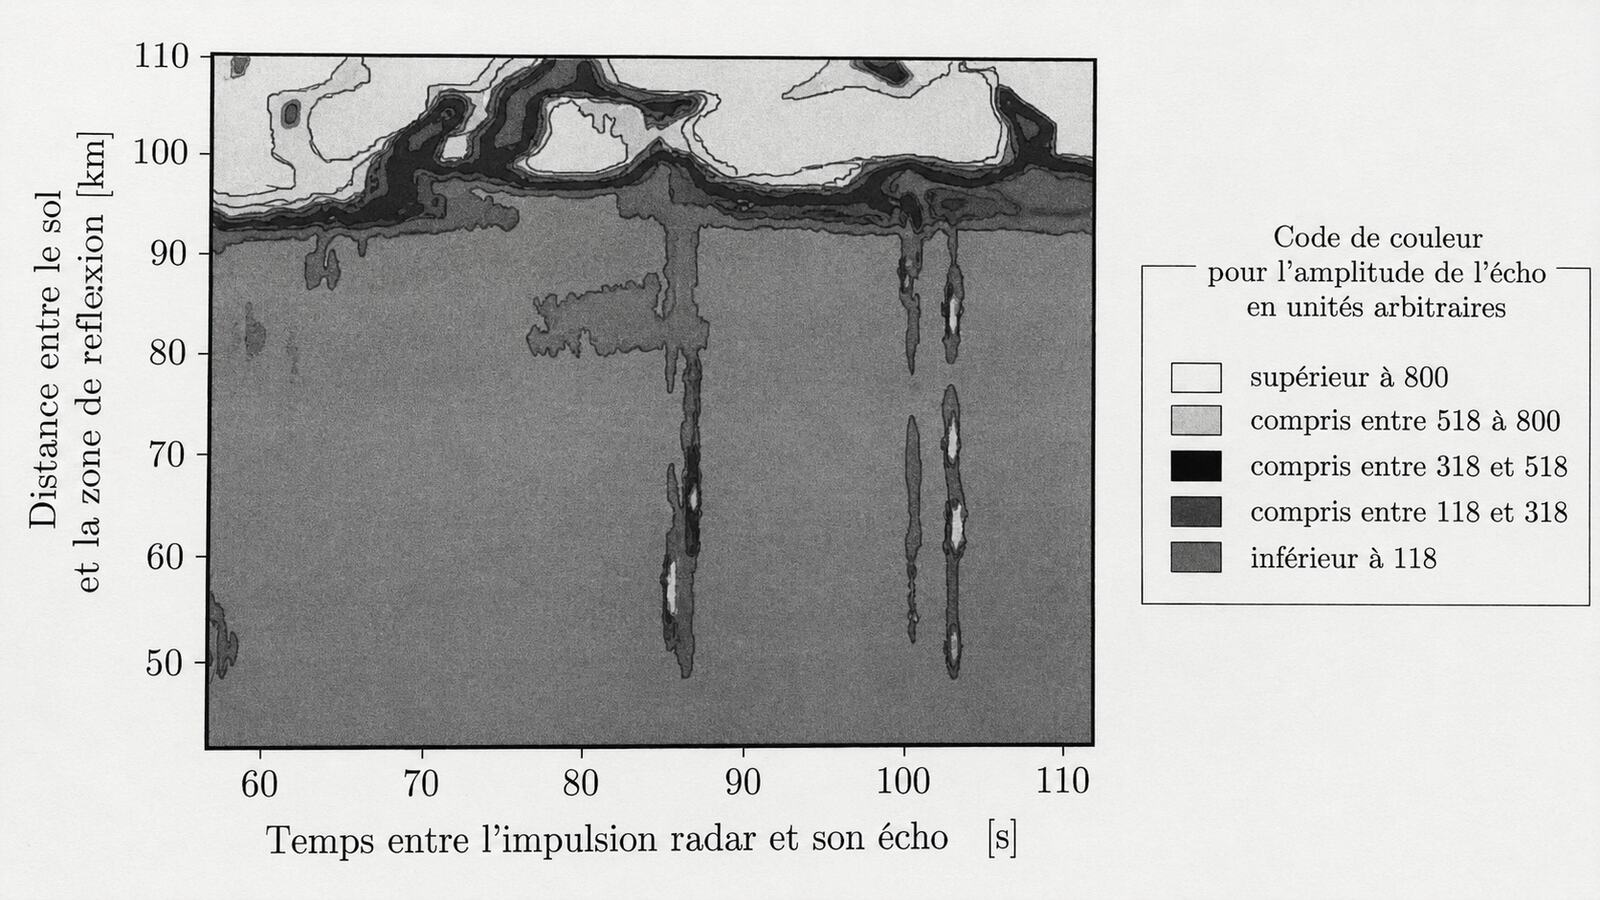
\includegraphics[width=0.86\linewidth]{figure_06.jpg}
\caption{Carte d'échos radar à 2,2~MHz depuis le sol pour l'événement enregistré à 13h39 le 15 octobre 1994 dans la station de Korhogo (Côte d'Ivoire). Figure tirée de l'article \textit{HF echoes from ionization potentially produced by high-altitude discharges}, R.~A.~Roussel-Dupré et E.~Blanc, \textit{Journal of Geophysical Research}, vol.~102, n\textsuperscript{o}~A3, p.~4613--4622, 1997.}
\label{fig:radar}
\end{figure}

\section*{III. Formation avalancheuse de courant}

L'origine des sylphes est toujours discutée à l'heure actuelle.
Un modèle repose sur la formation d'un courant lié à des ionisations en cascade provoquées par un électron primaire capable d'ioniser par chocs successifs des molécules de l'atmosphère, principalement du diazote \(\mathrm{N}_2\).
Les électrons fils créés par l'électron primaire peuvent à leur tour provoquer de nouvelles ionisations, d'où l'effet d'avalanche. Cet électron primaire peut provenir du rayonnement cosmique qui éclaire en permanence la Terre. Nous allons tout d'abord étudier la possibilité pour un tel électron de provoquer l'ionisation d'une molécule de diazote.

On considère un modèle unidimensionnel d'axe \(Ox\) où \(N_0\) électrons se déplacent de façon homogène dans le sens \(x\) croissant. Ces électrons sont répartis aléatoirement dans une section donnée \(\Sigma\). Leur déplacement s'effectue dans un milieu peu dense où la densité volumique de molécules est \(n_{\mathrm{mo}}\). On s'intéresse à la distance moyenne \(\langle x\rangle\) qu'ils vont parcourir avant de subir un choc avec une molécule. Cette distance porte le nom de libre parcours moyen : \(\ell_{\mathrm{pm}}=\langle x\rangle\). On appelle \(N(x)<N_0\) le nombre d'électrons qui ont atteint l'abscisse \(x\) sans subir de choc depuis \(x=0\). La probabilité qu'un électron subisse un choc entre les abscisses \(x\) et \(x+\mathrm{d}x\) est le rapport de la section efficace totale associée à l'ensemble des molécules présentes entre \(x\) et \(x+\mathrm{d}x\) et de la section \(\Sigma\). À chaque molécule est associée une section efficace \(S_{\mathrm{eff}}\), qui traduit le fait que si l'électron arrive sur cette surface, le choc se produit et s'il passe à côté, il n'y a pas de choc.

\question{18}
En raisonnant entre \(x\) et \(x+\mathrm{d}x\), établir l'équation différentielle d'évolution de \(N(x)\). Résoudre cette équation et exprimer \(N(x)\) en fonction de \(N_0\), \(n_{\mathrm{mo}}\), \(S_{\mathrm{eff}}\) et \(x\).

\question{19}
Montrer que le libre parcours moyen s'écrit
\[
\ell_{\mathrm{pm}}=\langle x\rangle=\frac{1}{n_{\mathrm{mo}}S_{\mathrm{eff}}}.
\]

\question{20}
Pour la molécule de diazote, on a \(S_{\mathrm{eff}}\simeq 10^{-20}~\mathrm{m}^2\). Justifier cet ordre de grandeur pour la section efficace. Déterminer la valeur numérique du libre parcours moyen \(\ell_{\mathrm{pm}}\) pour un électron à l'altitude \(z_3=60~\mathrm{km}\), où la pression est \(P_3=20~\mathrm{Pa}\) et la température \(T_3=260~\mathrm{K}\).

Au niveau des sylphes, il existe un champ électrique qui a pour principale origine les charges présentes à la surface des nuages d'une part et celles présentes à la limite entre la mésosphère et l'ionosphère vers 100~km d'altitude. Son intensité est \(E\simeq 100~\mathrm{V}\cdot\mathrm{m}^{-1}\).

\question{21}
Sachant que l'énergie d'ionisation de la molécule de diazote est \(\mathcal{E}_i\simeq 16~\mathrm{eV}\), un électron initialement au repos et accéléré par le champ électrique local d'intensité \(E\) peut-il ioniser cette molécule ? On apportera des arguments numériques.

On soupçonne fortement des électrons cosmiques relativistes possédant une énergie cinétique de 1~MeV d'être à l'origine de la cascade avalancheuse.

\question{22}
Justifier le fait que ces électrons cosmiques sont nécessairement relativistes.

\question{23}
Expliquer le phénomène de cascade avalancheuse.

On cherche à déterminer à partir de quel moment on atteint une densité moyenne \(n=10^{11}~\mathrm{m}^{-3}\) d'électrons caractéristique des sylphes. On note \(\mathcal{N}\) le nombre d'étapes produisant des électrons lors des chocs. Pour simplifier, on considère que tous les électrons produits jusqu'à l'étape \(\mathcal{N}\) sont contenus dans un volume dont la taille caractéristique est \(\mathcal{N}\ell_{\mathrm{pm}}\).

\question{24}
Déterminer la valeur numérique de \(\mathcal{N}\). Pour cette question, on prendra un libre parcours moyen \(\ell_{\mathrm{pm}}\) de l'ordre du centimètre. On pourra utiliser les courbes de la figure~\ref{fig:fonctions} en expliquant de façon détaillée la démarche suivie.

\begin{figure}[H]
\centering
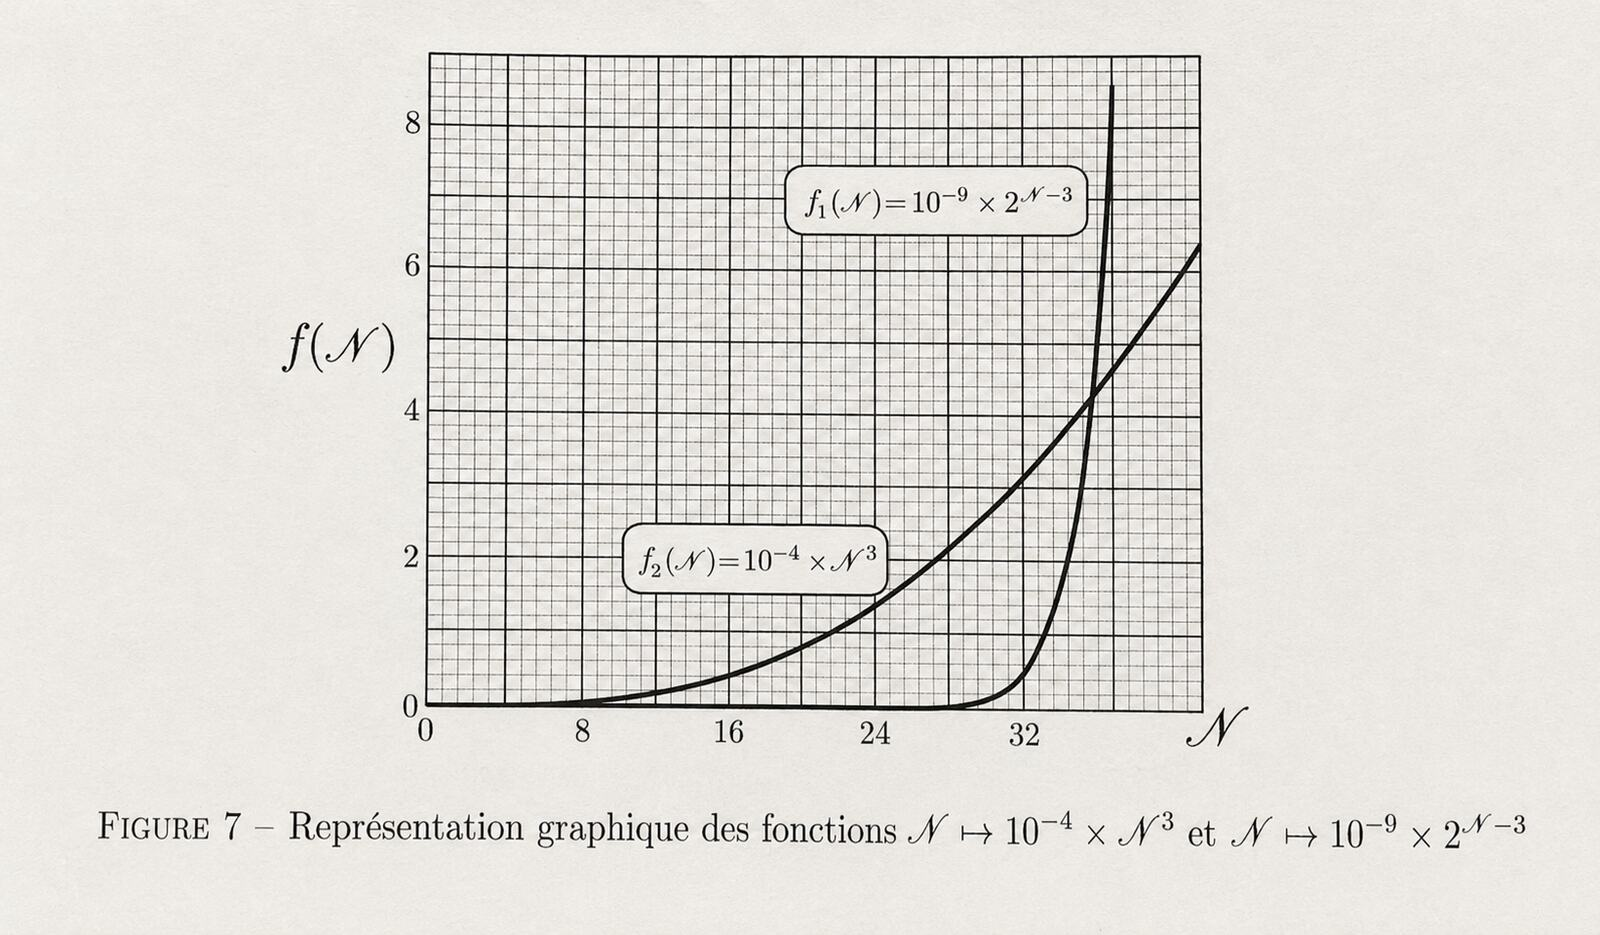
\includegraphics[width=0.72\linewidth]{figure_07.jpg}
\caption{Représentation graphique des fonctions \(\mathcal{N}\mapsto 10^{-4}\mathcal{N}^{3}\) et \(\mathcal{N}\mapsto 10^{-9}2^{\mathcal{N}-3}\).}
\label{fig:fonctions}
\end{figure}

\end{document}
